\documentclass[12pt,a4paper,twoside,openright,titlepage,final, svgnames]{book}
\usepackage{fontspec}
\usepackage{amsmath}
\usepackage{amsfonts}
\usepackage{amssymb}
\usepackage{makeidx}
\usepackage{graphicx}
\usepackage{minted}
\usepackage[hidelinks,unicode=true]{hyperref}
\usepackage[spanish,es-nodecimaldot,es-lcroman,es-tabla,es-noshorthands]{babel}
\usepackage[left=3cm,right=2cm, bottom=4cm]{geometry}
\usepackage{natbib}
\usepackage{microtype}
\usepackage{extras/tfg}
\usepackage{ifdraft}
\usepackage[obeyDraft]{todonotes}
\ifdraft{
	\usepackage{draftwatermark}
	\SetWatermarkText{BORRADOR}
	\SetWatermarkScale{0.7}
	\SetWatermarkColor{red}
}{}
\usepackage{booktabs}
\usepackage{longtable}
\usepackage{calc}
\usepackage{array}
\usepackage{caption}
\usepackage{subfigure}
\usepackage{footnote}
\usepackage{url}
\setsansfont[Ligatures=TeX]{texgyreadventor}
\setmainfont[Ligatures=TeX]{texgyrepagella}

\newcolumntype{C}[1]{>{\centering\arraybackslash}m{#1}}


\author{José Ignacio Escribano}

\usepackage{amsmath}
\usepackage{xparse}
\usepackage{amsthm}
\usepackage{tikz}

% Seno
\def\sen{\mathop{\mbox{\normalfont sen}}\nolimits}

% Seno hiperbólico
\def\senh{\mathop{\mbox{\normalfont senh}}\nolimits}

% Arcoseno
\def\arcsen{\mathop{\mbox{\normalfont arcsen}}\nolimits}

% Gradiente
\def\grad{\mathop{\mbox{\normalfont grad}}\nolimits}

% Argumento principal
\def\Arg{\mathop{\mbox{\normalfont Arg}}\nolimits}

% Logaritmo complejo
\def\Log{\mathop{\mbox{\normalfont Log}}\nolimits}

% Rotacional
\def\rot{\mathop{\mbox{\normalfont rot}}\nolimits}

% Divergencia
\def\diver{\mathop{\mbox{\normalfont div}}\nolimits}

% Longitud
\def\longi{\mathop{\mbox{\normalfont long}}\nolimits}

% Índice de una curva
\def\ind{\mathop{\mbox{\normalfont Ind}}\nolimits}

% Rango de una matriz
\def\rang{\mathop{\mbox{\normalfont rang}}\nolimits}

% Norma
\newcommand{\norm}[1]{\lVert #1 \rVert}

% Derivada parcial
\newcommand{\derpar}[1]{\dfrac{\partial}{\partial #1}}

% Derivada parcial con función
\newcommand{\derparcial}[2]{\dfrac{\partial #1}{\partial #2}}

% Derivada parcial de orden n con funcion
\newcommand{\derparcialn}[3]{\dfrac{\partial^{#3} #1}{\partial #2^{#3}}}

% Integral doble en [a,b] x [c,d]
\newcommand{\intdob}[4]{\displaystyle \int_{#1}^{#2} \int_{#3}^{#4}}

% Integral triple en [a,b] x [c,d] x [e,f]
\newcommand{\inttri}[6]{\displaystyle \int_{#1}^{#2} \int_{#3}^{#4} \int_{#5}^{#6}}

% Números complejos
\def\C{\ensuremath{\mathbb{C}}}

% Números reales
\def\R{\ensuremath{\mathbb{R}}}

% Números racionales
\def\Q{\ensuremath{\mathbb{Q}}}

% Números enteros
\def\Z{\ensuremath{\mathbb{Z}}}

% Números naturales
\def\N{\ensuremath{\mathbb{N}}}

% Teorema
\newtheorem{teo}{Teorema}

% Corolario
\newtheorem{cor}{Corolario}

% Proposición
\newtheorem{prop}{Proposición}

% Lema
\newtheorem{lema}{Lema}

% Definición
\newtheorem{defi}{Definición}

% Observaciones
\newtheorem*{obs}{Observaciones}

\newtheorem*{ob}{Observación}

\newtheorem*{nota}{Nota}

\newtheorem*{problema}{Problema}

\newtheorem*{pregunta}{Pregunta}

\newtheorem{ejemplo}{Ejemplo}

\NewDocumentCommand{\overarrow}{O{=} O{\uparrow} m}{%
  \overset{\makebox[0pt]{\begin{tabular}{@{}c@{}}#3\\[0pt]\ensuremath{#2}\end{tabular}}}{#1}
}
\NewDocumentCommand{\underarrow}{O{=} O{\downarrow} m}{%
  \underset{\makebox[0pt]{\begin{tabular}{@{}c@{}}\ensuremath{#2}\\[0pt]#3\end{tabular}}}{\ensuremath{#1}}
}

\newcommand{\contradiction}{%
\begin{tikzpicture}[rotate=45,x=0.5ex,y=0.5ex]
\draw[color=red, line width=.1ex] (0,2) -- (3,2) (0,1) -- (3,1) (1,3) -- (1,0) (2,3) -- (2,0);
\end{tikzpicture}
}

%*******************************************************
%                 NO MODIFICAR
\newcommand*{\FSfont}[1]{%
	\fontencoding{T1}\fontfamily{#1}\selectfont}

\newlength{\tpheight}\setlength{\tpheight}{0.9\textheight}
\newlength{\txtheight}\setlength{\txtheight}{0.9\tpheight}
\newlength{\tpwidth}\setlength{\tpwidth}{0.9\textwidth}
\newlength{\txtwidth}\setlength{\txtwidth}{0.9\tpwidth}
\newlength{\drop}
%*******************************************************

% Crea una portada con los siguientes parámetros
%
% #1 : Título 
% #2 : Subtítulo
% #3 : Autor(es)
% #4 : Tutor(es)
% #5 : Lugar
%

\newcommand*{\portada}[5]{
	\begin{titlepage}
		\begingroup
		%\vspace*{1cm}
		\drop = 0.2\txtheight
		\centering
		\vspace*{0.5cm}
		
\includegraphics[scale=0.8]{./imagenes/logo-urjc}

		\vspace*{1.5cm}
		{\Huge  \textbf{#1}}\\[\baselineskip]
		{\Large{Trabajo Fin de Grado}}\\[\baselineskip]
		
		{\large {Escuela Técnica Superior de Ingeniería Informática}}\\[\baselineskip]
		
		\vspace*{0.5cm}
		
		{\large \textbf{#2}}\\[\baselineskip]
		
		{\large{#3}}\\[\baselineskip]
		
		\vspace*{0.5cm}
		
		{\large \textit{#4}}\\[0.5\drop]
		
		\vspace*{0.5cm}
		
		{Tutores:} \\ 
		{\large \textit{#5}}
		\begin{center}
		\end{center}
		\vfill\null
		\endgroup
	\end{titlepage}
}
%*****************************************************


\usepackage{pgf}
\usepackage{tikz}
\usetikzlibrary{arrows,automata}

\newcommand{\ejemplografo}{
\begin{tikzpicture}[>=stealth',shorten >=1pt,auto,node distance=3cm,semithick]
  \tikzstyle{every state}=[draw=black,text=black]

  \node[state]         (A)                    {$A$};
  \node[state]         (B) [right of=A]       {$B$};
  \node[state]         (C) [below of=A]       {$C$};
  \node[state]         (D) [right of=C]       {$D$};
  
  \path (A) edge  [bend left]   node {}  (B)
            edge  [bend right]  node {}  (C)
        (B) edge                node {}  (C)
        (C) edge  [bend right]  node {}  (D);
\end{tikzpicture}}

\newcommand{\ejemplografocompleto}{
\begin{tikzpicture}[>=stealth',shorten >=1pt,auto,node distance=3cm,semithick]
  \tikzstyle{every state}=[draw=black,text=black]

  \node[state]         (A)                    {$A$};
  \node[state]         (B) [right of=A]       {$B$};
  \node[state]         (C) [below of=A]       {$C$};
  \node[state]         (D) [right of=C]       {$D$};
  
  \path (A) edge  [bend left]   node {}  (B)
            edge  [bend right]  node {}  (C)
		(B) edge  [bend left]   node {}  (D)
        (B) edge                node {}  (C)
        (D) edge                node {}  (A)
        (C) edge  [bend right]  node {}  (D);
\end{tikzpicture}}

\newcommand{\ejemplografodirigido}{
\begin{tikzpicture}[->,>=stealth',shorten >=1pt,auto,node distance=3cm,semithick]
  \tikzstyle{every state}=[draw=black,text=black]

  \node[state]         (A)                    {$A$};
  \node[state]         (B) [right of=A]       {$B$};
  \node[state]         (C) [below of=A]       {$C$};
  \node[state]         (D) [right of=C]       {$D$};
  
  \path (A) edge  [bend left]   node {}  (B)
            edge  [bend right]  node {}  (C)
        (B) edge                node {}  (C)
        (C) edge  [bend right]  node  {}  (D)
        (C) edge  [loop below]  node  {}  (C);
\end{tikzpicture}}

\newcommand{\ejemplosubgrafo}{
\begin{tikzpicture}[>=stealth',shorten >=1pt,auto,node distance=2cm,semithick]
  \tikzstyle{every state}=[draw=black,text=black]

% Grafo G
  \node[state]         (E)                          {$E$};
  \node[state]         (B) [above right of=E]       {$B$};
  \node[state]         (A) [above left of= E]       {$A$};
  \node[state]         (C) [below left of= E]       {$C$};
  \node[state]         (D) [below right of=E]       {$D$};

  \path (A) edge                node {}  (B)
        (A) edge                node {}  (E)
        (A) edge                node {}  (C)
        (B) edge                node {}  (D)
        (B) edge                node {}  (E)        
        (C) edge                node {}  (E)
        (C) edge                node {}  (D)
        (D) edge                node {}  (E);
        
        
% Subgrafo G'
  \node[state]         (F) [right of= B]       {$A$};
  \node[state]         (G) [right of= F]       {$B$};
  \node[state]         (H) [right of= D]       {$C$};
  \node[state]         (I) [right of= H]       {$D$};
  
  \path (F) edge                node {}  (G)
        (F) edge                node {}  (H)
        (G) edge                node {}  (I)
        (H) edge                node {}  (I);
        
% Subgrafo G'

  \node[state]         (J) [right of= G]             {$A$};
  \node[state]         (K) [right of= I]             {$C$};
  \node[state]         (N) [above right of= K]       {$E$};
  \node[state]         (M) [below right of= N]       {$D$};
  \node[state]         (L) [above right of= N]       {$B$};
  
  \path (J) edge                node {}  (K)
        (J) edge                node {}  (L)
        (L) edge                node {}  (N)
        (L) edge                node {}  (M)
        (K) edge                node {}  (M);
        
% Etiquetas con el nombre de los grafos
  \node[align=center, below right of=C] {$G$};
  \node[align=center, below right of=H] {$G'$};
  \node[align=center, below right of=K] {$G''$};
\end{tikzpicture}}

\newcommand{\ejemplounionintersecciongrafo}{
\begin{tikzpicture}[>=stealth',shorten >=1pt,auto,node distance=2cm,semithick]
  \tikzstyle{every state}=[draw=black,text=black]

% Grafo G
  \node[state]         (A)                          {$A$};
  \node[state]         (B) [below right of=A]       {$B$};
  \node[state]         (C) [below      of= B]       {$C$};
  \node[state]         (D) [right of=B]             {$D$};
  \node[state]         (E) [right of=C]             {$E$};

  \path (A) edge                node {}  (B)
        (B) edge                node {}  (C)
        (B) edge                node {}  (D)      
        (C) edge                node {}  (E)
        (D) edge                node {}  (E);
        
% Grafo G'
  \node[state]         (H) [right of= E]       {$C$};
  \node[state]         (I) [right of= D]       {$D$};
  \node[state]         (G) [right of= H]       {$E$};
  \node[state]         (F) [above right of= G] {$F$};
  
  \path (H) edge                node {}  (I)
        (I) edge                node {}  (F)
        (G) edge                node {}  (F)
        (H) edge                node {}  (G);
        
% Etiquetas con el nombre de los grafos
  \node[align=center, below right of=C] (Z) {$G$};
  \node[align=center, below right of=H] (Y) {$G'$};

% Grafo G \cup G'
  \node[state]         (J) [below left of=Z]        {$A$};
  \node[state]         (K) [below right of=J]       {$B$};
  \node[state]         (L) [below of= K]            {$C$};
  \node[state]         (M) [right of=K]             {$D$};
  \node[state]         (N) [right of=L]             {$E$};
  \node[state]         (R) [above right of=N]       {$F$};

  \path (J) edge                node {}  (K)
        (K) edge                node {}  (L)
        (K) edge                node {}  (M)      
        (L) edge                node {}  (N)
        (L) edge                node {}  (M)
        (N) edge                node {}  (R)
        (R) edge                node {}  (M)
        (M) edge                node {}  (N);
        
  \node[align=center, below right of=L] {$G \cup G'$};
  
% Grafo G \cup G'
  \node[state]         (O) [right of=R]        {$C$};
  \node[state]         (P) [right of=O]              {$E$};


  \path (O) edge                node {}  (P);
        
        
  \node[align=center, below right of=O] {$G \cap G'$};

\end{tikzpicture}}


\newcommand{\ejemplomarkov}{
\begin{tikzpicture}[->,>=stealth',shorten >=1pt,auto,node distance=5cm,semithick]
  \tikzstyle{every state}=[draw=black,text=black]

  \node[state]         (A)                    {$A$};
  \node[state]         (B) [below left of=A]  {$B$};
  \node[state]         (C) [below right of=A] {$C$};
  
  \path (A) edge  [loop above] node {$0.65$} (A)
            edge  [bend left]  node {$0.3$}  (B)
            edge  [bend left]  node {$0.05$} (C)
        (B) edge  [loop below] node {$0.75$} (B)
            edge  [bend left]  node {$0.1$}  (A)
            edge               node {$0.15$} (C)
        (C) edge  [loop below] node {$0.8$}  (C)
            edge  [bend left]  node {$0.01$} (A)
            edge  [bend left]  node {$0.19$} (B);
\end{tikzpicture}}

\newcommand{\ejemplomarkovcompleto}{
\begin{tikzpicture}[->,>=stealth',shorten >=1pt,auto,node distance=5cm,semithick]
  \tikzstyle{every state}=[draw=black,text=black]

  \node[state]         (S)                    {$S$};
  \node[state]         (H)      [right of=A]  {$H$};
  
  \path (S) edge  [loop above] node {$0.5$}  (S)
            edge  [bend left]  node {$0.5$}  (H)
        (H) edge  [loop below] node {$0.75$} (H)
            edge  [bend left]  node {$0.25$} (S);

\end{tikzpicture}}



\setlength{\parindent}{0pt}

\begin{document}
\frontmatter
\portada{TFG Software}{Título}{ \ }{José Ignacio Escribano}{Móstoles}
\tableofcontents
\listoffigures
\listoftables

\mainmatter
\chapter{Introducción}
\chapter{Conceptos básicos de rankings} \label{chp:conceptos_basicos}

En este capítulo veremos dos de los conceptos claves de esta memoria: ranking y rating, que darán lugar a cómo estudiar la competitividad en los rankings.\\

Para entender estos conceptos, comencemos con un ejemplo:

\begin{ejemplo}
Consideremos el número de goles, los partidos jugados y el promedio de goles de Messi (MES), Cristiano Ronaldo (CRO) y Raúl González (RAU) en la UEFA Champions League.

\begin{table}[h]
\centering
\caption[Goles, partidos jugados de los máximos goleadores de la Champions]{Goles, partidos jugados y promedio de goles de los máximos goleadores de la Champions}
\label{tbl:goles_champions}

\begin{tabular}{cccc}
\cline{2-4}
    & Goles & Partidos jugados & Promedio goleador \\ \cline{2-4} 
MES & 77    & 97               & 0.79              \\
CRO & 77    & 115              & 0.67              \\
RAU & 71    & 142              & 0.5               \\ \hline
\end{tabular}
\end{table}


Estas tres estadísticas del juego (goles, partidos jugados y promedio) pueden dar lugar a distintas ordenaciones de los jugadores. Por ejemplo, si consideramos el número de goles o el promedio goleador, el ranking de estos tres jugadores quedaría de la siguiente manera:

\[
\begin{array}{cc}
\text{Posición} & \text{Goles}\\ 
\begin{array}{c}
\text{1}\\
\text{2}\\
\text{3}
\end{array} & \left(\begin{array}{c}
\text{MES}\\
\text{CRO}\\
\text{RAU}
\end{array} \right)
\end{array}
\] 

Sin embargo, si consideramos el número de partidos jugados en la UEFA Champions League, el ranking quedaría de la siguiente manera:

\[
\begin{array}{cc}
\text{Posición} & \text{Partidos jugados}\\ 
\begin{array}{c}
\text{1}\\
\text{2}\\
\text{3}
\end{array} & \left(\begin{array}{c}
\text{RAU}\\
\text{CRO}\\
\text{MES}
\end{array} \right)
\end{array}
\] 

Vemos, que distintos parámetros pueden dar lugar a diferentes rankings.

\end{ejemplo}


Un rating, de forma intuitiva, es un criterio de ordenación de un conjunto de elementos; y un ranking es una posible ordenación de un conjunto de elementos.\\

Veamos las definiciones rigurosas de estos dos conceptos:

\begin{defi} \label{def:ranking}
Dado un conjunto $\mathcal{N} = \{1,\dots,n\}$ que llamamos nodos, definimos el ranking $c$ como cualquier biyección $c : \mathcal{N} \to \mathcal{N}$.
\end{defi}

\begin{defi}
Dado un conjunto $\mathcal{N} = \{1,\dots, n\}$ de nodos, decimos que es un rating si a cada $i \in \mathcal{N}$ se le asigna un valor real, es decir, una función $\mathrm{r} : \mathcal{N} \to \R$.
\end{defi}

De acuerdo a estas dos definiciones, podemos definir $\mathcal{N} = \{1,2,3 \}$ donde MES $\equiv 2$, CRO $\equiv 3$ y RAU $\equiv 1$. De esta forma podemos ver el ranking de goles como la biyección $c: \mathcal{N} \to \mathcal{N}$ definida de la siguiente manera:

\[ \begin{array}{rlll}
c: & \mathcal{N} & \to & \mathcal{N}\\
& 1 & \mapsto & 2\\
& 2 & \mapsto & 3\\
& 3 & \mapsto & 1
\end{array} \] 

Por lo que efectivamente, se trata de un ranking.\\

Para el promedio de goles, podemos definir la función $r : \mathcal{N} \to \R$ definida de la siguiente manera:

\[ \begin{array}{rlll}
c: & \mathcal{N} & \to & \R\\
& 2 & \mapsto & 0.97\\
& 3 & \mapsto & 0.67\\
& 1 & \mapsto & 0.50
\end{array} \] 

Por lo que se cumple que es un rating.\\

Además, escribiremos $i \prec_c j$ cuando el nodo $i \in \mathcal{N}$ aparezca antes que el nodo $j \in \mathcal{N}$ en el ranking $c$.\\

Si volvemos al ejemplo anterior, se tiene que $2 \prec_c 3$, puesto que el nodo $2$ (MES) aparece antes que en el nodo $3$ en el ranking $c$.\\

Existen diversos modos para obtener rankings que se basan en distintos conceptos como mínimos cuadrados o cadenas de Markov. Estos métodos se pueden consultar en~\cite{langville2012s}.

\section{Competitividad en rankings}

Uno de los aspectos más interesantes de los rankings, es la competitividad. Cuando se dispone de una gran cantidad de rankings, es interesante ver cómo se van intercambiando las posiciones los equipos. De esta forma estudiaremos la competitividad en los rankings. Los cambios de posiciones de los equipos darán lugar a dos nuevos tipos de grafos (grafo de competitividad y grafo de competitividad evolutivo). Una introducción a la teoría de grafos se puede encontrar en el Anexo~\ref{teoria_grafos}.\\

Empezamos definiendo la competitividad entre una familia de rankings.

\begin{defi}
Dada una familia $\mathcal{R} = \{c_1, c_2, \dots, c_r\}$ de rankings, 
 $(i,j) \in \mathcal{N} \times \mathcal{N}$ compiten si existe $t \in \{1,2,\dots, r-1\}$ tal que $i$ y $j$ intercambian sus posiciones relativas entre rankings consecutivos $c_t$ y $c_{t+1}$.
\end{defi}

\begin{ejemplo}
Si consideramos la familia de rankings $\mathcal{R} = \{c_1, c_2\}$ donde $c_1$ y $c_2$ son, respectivamente

\begin{equation*}
c_1 = \left( \begin{array}{c}
1\\
3\\
2\\
4\\
5
\end{array} \right), \quad
c_2 = \left( \begin{array}{c}
1\\
2\\
4\\
3\\
5
\end{array} \right)
\end{equation*}

Los pares $(1,2)$ y $(1,3)$ no compiten, puesto que los nodos no intercambian sus posiciones relativas entre rankings consecutivos. Sin embargo, los pares $(3,4)$ y $(2,3)$ sí compiten puesto que intercambian sus posiciones relativas entre rankings consecutivos, $c_1$ y $c_2$.
\end{ejemplo}  

\subsection{Grafo de competitividad}

Los pares de nodos que compiten dan lugar a un grafo, que llamaremos grafo de competitividad. Este grafo tiene propiedades interesantes como veremos a continuación.

\begin{defi}[Grafo de competitividad]
Definimos grafo de competitividad de la familia de rankings $\mathcal{R}$, y lo denotaremos como $G_c(\mathcal{R}) = (\mathcal{N}, E_\mathcal{R})$, donde $\mathcal{N}$ es el conjunto de nodos $E_\mathcal{R}$ denota el conjunto de arcos dados por la siguiente regla: existe un arco entre $i$ y $j$ si el par $(i,j)$ compite.
\end{defi}

\begin{ejemplo} \label{ej:grafo_competitividad}
Consideremos la familia de rankings $\mathcal{R} =\{c_1, c_2, c_3, c_4\}$ formada por cuatro clasificaciones ficticias de los equipos Real Madrid (RMA), Barcelona (BAR), Sevilla (SEV) y Valencia (VAL). Las cuatro clasificaciones son las siguientes:

\begin{equation*}
c_1 = \left( \begin{array}{c}
\text{RMA}\\
\text{BAR}\\
\text{SEV}\\
\text{VAL}
\end{array} \right), \quad
c_2 = \left( \begin{array}{c}
\text{RMA}\\
\text{SEV}\\
\text{VAL}\\
\text{BAR}
\end{array} \right), \quad
c_3 = \left( \begin{array}{c}
\text{RMA}\\
\text{BAR}\\
\text{VAL}\\
\text{SEV}
\end{array} \right), \quad
c_4 = \left( \begin{array}{c}
\text{RMA}\\
\text{VAL}\\
\text{BAR}\\
\text{SEV}
\end{array} \right)
\end{equation*}

La Figura~\ref{fig:grafo_competitividad} muestra el grafo de competitividad de la familia de rankings $\mathcal{R}$. El grafo tiene dos componentes conexas: $\{\text{BAR}, \text{SEV}, \text{VAL}\}$ y $\{\text{RMA}\}$. Vemos que hay pares de equipos que compiten más de una vez, por ejemplo, el par $(\text{BAR}, \text{VAL})$ cambian sus posiciones relativas tres veces en los rankings $c_1$, $c_2$, $c_3$ y $c_4$. Esta información no la recoge el grafo de competitividad. Esta información la recogerá el grafo de competitividad evolutivo. 

\begin{figure}[htb]
\centering
\ejemplografocompetitividad
\caption[Grafo de competitividad]{Grafo de competitividad de $\mathcal{R}$}
\label{fig:grafo_competitividad}
\end{figure}

\end{ejemplo}

\begin{defi}
Decimos que los nodos $i$, $j$ compiten $k$ veces si $k$ es el número máximo de veces de rankings que $i$ y $j$ compiten.
\end{defi}

\begin{defi}
El grafo de competitividad evolutivo de $\mathcal{R}$, denotado por $G_c^e(\mathcal{R}) = (\mathcal{N}, E_\mathcal{R}^e)$ es el grafo ponderado con el conjunto $\mathcal{N}$ como nodos y aristas dadas por la siguiente regla: hay una arista entre $i$ y $j$ con peso $k$ si $(i,j)$ compiten $k$ veces.
\end{defi}

\begin{ejemplo}
Consideramos de nuevo la familia $\mathcal{R}$ de rankings del Ejemplo \ref{ej:grafo_competitividad}. El grafo de competitividad de $\mathcal{R}$ se muestra en la Figura~\ref{fig:grafo_competitividad_evolutivo}.

\begin{figure}[htb]
\centering
\ejemplografocompetitividadevolutivo
\caption[Grafo de competitividad evolutivo]{Grafo de competitividad evolutivo de $\mathcal{R}$}
\label{fig:grafo_competitividad_evolutivo}
\end{figure}

\end{ejemplo}

Notar que si eliminamos los pesos del grafo de competitividad evolutivo, obtenemos el grafo de competitividad.

\section{Medidas de competitividad}

Cuando se dispone de más de una familia de rankings, es necesario disponer de una serie de medidas que permitan medir la competitividad en cada uno de los grafos de competitividad. Algunas de estas medidas son grado medio normalizado, fuerza media normalizada y una generalización de la tau de Kendall para una familia de rankings.

\subsection*{Grado medio normalizado}

\begin{defi}
Se define grado medio normalizado de una familia de rankings $\mathcal{R}$, como la suma de todos los grados de los nodos en el grafo de competitividad $G_c(\mathcal{R})$ dividido por la suma sobre todos los nodos de sus grados más altos posibles. Esto es,

\begin{equation}
\mathrm{ND}(\mathcal{R}) = \dfrac{1}{n(n-1)} \sum_{i \in \mathcal{N}} d_i
\end{equation}

donde $d_i$ es el número de nodos adyacentes al nodo  $i$.
\end{defi}

\begin{defi}
Se dice que la familia de rankings $\mathcal{R}$ es más competitiva que la familia de rankings $\mathcal{S}$ con respecto al grado medio normalizado si $\mathrm{ND}(\mathcal{R}) > \mathrm{ND}(\mathcal{S})$.
\end{defi}

\begin{ejemplo}
Consideremos la familia de rankings $\mathcal{R}$ y el grafo de competitividad del Ejemplo~\ref{ej:grafo_competitividad} y el grafo de competitividad $G_c(\mathcal{S})$ de la Figura~\ref{fig:grado_medio}.\\

\begin{figure}[htb]
\centering
\ejemplogradomedio
\caption{Grafo de competitividad de $\mathcal{S}$}
\label{fig:grado_medio}
\end{figure}

El grado medio de las dos familias son:

\begin{eqnarray*}
\mathrm{ND}(\mathcal{R}) = \dfrac{1}{4\cdot 3} (0 + 2 + 2 + 2) = \dfrac{6}{12} = \dfrac{1}{2}\\
\mathrm{ND}(\mathcal{S}) = \dfrac{1}{4\cdot 3} (2 + 3 + 1 + 2) = \dfrac{8}{12} = \dfrac{2}{3}
\end{eqnarray*}

Puesto que $\mathrm{ND}(\mathcal{S}) > \mathrm{ND}(\mathcal{R})$, la familia $\mathcal{S}$ es más competitiva que la familia $\mathcal{R}$ con respecto al grado medio normalizado.
\end{ejemplo}

\subsection*{Fuerza media normalizada}

\begin{defi}
Se define la fuerza media normalizada de una familia de rankings $\mathcal{R}$ como la suma de todos pesos de las aristas del grafo de competitividad evolutivo $G_c^e(\mathcal{R})$ dividido entre la suma de todas las posibles aristas con sus máximos pesos posibles. Esto es,

\begin{equation}
\mathrm{NS}(\mathcal{R}) = \dfrac{w(E_\mathcal{R}^e)}{\binom{n}{2} (r-1)}
\end{equation} 

donde $w(E_\mathcal{R}^e)$ denota la suma de todos los pesos de las aristas del grafo de competitividad evolutivo $G_c^e(\mathcal{R})$ y $r$ es el número de rankings de la familia $\mathcal{R}$.
\end{defi}

\begin{defi}
Se dice que $\mathcal{R}$ es más competitivo que $\mathcal{S}$ con respecto a la fuerza media normalizada si $\mathrm{NS}(\mathcal{R}) > \mathrm{NS}(\mathcal{S})$.
\end{defi}

\begin{ejemplo}
Consideremos la familia $\mathcal{R}$ del Ejemplo~\ref{ej:grafo_competitividad} y el grafo de competitividad evolutivo de la familia $\mathcal{S}$ compuesta por $4$ rankings de la Figura~\ref{fig:grado_medio}.\\

Calculamos la fuerza media de cada una de las familias de rankings,

\begin{eqnarray*}
\mathrm{NS}(\mathcal{R}) = \dfrac{6}{6 \cdot 3} = \dfrac{1}{3}\\
\mathrm{NS}(\mathcal{S}) = \dfrac{5}{6 \cdot 3} = \dfrac{5}{18}
\end{eqnarray*}

Como $\mathrm{NS}(\mathcal{R}) > \mathrm{NS}(\mathcal{S})$, la familia de rankings $\mathcal{R}$ es más competitiva con respecto a la fuerza media normalizada que la familia $\mathcal{S}$.

\end{ejemplo}

\subsection*{Tau de Kendall generalizada}

\begin{defi}
Llamamos tau de Kendall entre dos rankings $c_1$ y $c_2$ con $n$ elementos cada uno al siguiente valor

\begin{equation}
\tau(c_1, c_2) = \dfrac{\tilde{K}(c_1, c_2) - K(c_1, c_2)}{\binom{n}{2}}
\end{equation} 

donde $\tilde{K}(c_1, c_2)$ es el número de pares $(i,j)$ que no compiten con respecto a $\mathcal{R} = \{c_1, c_2\}$, y $K(c_1, c_2)$ denota el número de pares que compiten en $\mathcal{R}$.
\end{defi}

Esta medida de dos rankings se puede generalizar a una familia con $r$ rankings de la siguiente forma.

\begin{defi}
Se define tau de Kendall generalizada a la familia de rankings $\mathcal{R}$, con $r \geq 2$ de la siguiente manera:

\begin{equation}
\tau(\mathcal{R}) = \dfrac{\tilde{K}(c_1, c_2) - K(c_1, c_2)}{\binom{n}{2}} = 1 - \dfrac{4 |E_\mathcal{R}|}{n(n-1)}
\end{equation}

donde $|E_\mathcal{R}|$ es el número de aristas del grafo de competitividad $G_c(\mathcal{R})$.
\end{defi}

\begin{defi}
Se define tau de Kendall evolutiva de la familia de rankings $\mathcal{R}$ con $r \geq 2$ rankings de la siguiente manera:

\begin{equation}
\tau_e(\mathcal{R}) = 1 - \dfrac{2 w(E_\mathcal{R}^e)}{\binom{n}{2}(r-1)}
\end{equation} 

donde $w(E_\mathcal{R}^e)$ denota la suma sobre todos las aristas de sus pesos máximos posibles del grafo de competitividad evolutivo.
\end{defi}

\begin{defi}
Decimos que la familia de rankings $\mathcal{R}$ es más competitiva con respecto a la tau de Kendall evolutiva que la familia de rankings $\mathcal{S}$ si $\tau_e(\mathcal{R}) < \tau_e(\mathcal{S})$.
\end{defi}

\begin{ejemplo}
Consideremos los grafos evolutivos de las Figuras~\ref{fig:grafo_competitividad_evolutivo}~y~\ref{fig:grado_medio}. Calculamos la tau de Kendall para la familia de rankings $\mathcal{R}$.

\begin{eqnarray}
\tau(\mathcal{R}) = 1 - \dfrac{1}{2} = \dfrac{1}{2}\\
\tau_e(\mathcal{R}) = 1 - \dfrac{112}{12} = 1
\end{eqnarray}

De la misma forma para la familia $\mathcal{S}$,

\begin{eqnarray}
\tau(\mathcal{S}) = 1 - \dfrac{16}{12} = -\dfrac{1}{3}\\
\tau_e(\mathcal{S}) = 1 - \dfrac{8}{9} = \dfrac{1}{9}
\end{eqnarray}

Como $\tau_e(\mathcal{S}) < \tau_e(\mathcal{R})$ se tiene que la familia $\mathcal{S}$ es más competitiva que la familia $\mathcal{S}$ con respecto a la tau de Kendall.

\end{ejemplo}

\subsection*{Diámetro del grafo de competitividad evolutivo}

\begin{defi}
Se define diámetro del grafo de competitividad evolutivo de la familia de rankings $\mathcal{R}$ de la siguiente forma:

\begin{equation}
\mathrm{diam}(\mathcal{R}) = \max \{ d(i,j) : i \neq j \}
\end{equation}

donde $d(i,j)$ es la distancia entre el nodo $i$ y el nodo $j$.
\end{defi}

\begin{defi}
Diremos que la familia de rankings $\mathcal{R}$ es más competitiva que la familia de rankings $\mathcal{S}$ con respecto al diámetro del grafo de competitividad evolutivo si $\mathrm{diam}(\mathcal{R}) < \mathrm{diam}(\mathcal{S})$.
\end{defi}

\begin{ejemplo}
Consideremos los grafos evolutivos de las Figuras~\ref{fig:grafo_competitividad_evolutivo}~y~\ref{fig:grado_medio}. Calculemos el diámetro para la familia de rankings $\mathcal{R}$ y la familia $\mathcal{S}$.\\

Necesitamos calcular la distancia entre todos los pares de vértices y coger el máximo. Para ello, aplicamos el algoritmo de Floyd-Warshall.\\

En el caso de la familia $\mathcal{R}$ de rankings, obtenemos que la matriz de distancias tras la ejecución del algoritmo, es:


\begin{equation*}
\bordermatrix{
	& \text{RMA} & \text{BAR} & \text{VAL} & \text{SEV} \cr
	\text{RMA} &	0 & \infty & \infty & \infty \cr
	\text{BAR} & \infty & 0 & 3 & 2 \cr
	\text{VAL} & \infty & 3 & 0 & 1 \cr
	\text{SEV} & \infty & 2 & 1 & 0 \cr
}
\end{equation*}


donde, por convenio, $\infty$ significa que no existe un camino que permita llegar a esos dos nodos.\\

Por lo tanto,

\begin{equation*}
\mathrm{diam}(\mathcal{R}) = \infty
\end{equation*}

Para la familia $\mathcal{S}$ de rankings, tenemos que la matriz de distancias es la siguiente:

\begin{equation*}
\bordermatrix{
	& \text{RMA} & \text{BAR} & \text{VAL} & \text{SEV} \cr
	\text{RMA} & 0 & 1 & 2 & 2 \cr
	\text{BAR} & 1 & 0 & 1 & 1 \cr
	\text{VAL} & 2 & 1 & 0 & 2 \cr
	\text{SEV} & 2 & 1 & 2 & 0 \cr
}
\end{equation*}

Por tanto, 

\begin{equation*}
\mathrm{diam}(\mathcal{S}) = 2
\end{equation*}

Como $\mathrm{diam}(\mathcal{S}) < \mathrm{diam}(\mathcal{R})$, la familia $\mathcal{S}$ es más competitiva que la familia $\mathcal{R}$ con respecto al diámetro del grafo de competitividad evolutivo.

\end{ejemplo}

\subsection*{Eficiencia del grafo de competitividad evolutivo}

\begin{defi}
Se define eficiencia del grafo de competitividad evolutivo de la familia de rankings $\mathcal{R}$ de la siguiente forma:

\begin{equation}
\mathrm{E}(\mathcal{R}) = \dfrac{1}{\binom{n}{2}} \sum_{i\neq j} \dfrac{1}{d(i,j)}
\end{equation}

donde $d(i,j)$ es la distancia entre el nodo $i$ y el nodo $j$.
\end{defi}

La eficiencia es la media armónica de todos los caminos del grafo de competitividad.

\begin{defi}
Diremos que la familia de rankings $\mathcal{R}$ es más competitiva que la familia de rankings $\mathcal{S}$ con respecto a la eficiencia del grafo de competitividad evolutivo si $\mathrm{E}(\mathcal{R}) > \mathrm{E}(\mathcal{S})$.
\end{defi}

\begin{ejemplo}
Consideremos los grafos evolutivos de las Figuras~\ref{fig:grafo_competitividad_evolutivo}~y~\ref{fig:grado_medio}. Calculemos la eficiencia para la familia de rankings $\mathcal{R}$ y la familia $\mathcal{S}$.\\

En el ejemplo anterior ya calculamos la matriz de distancias de cada una de las familias, por lo que no es necesario volver a calcularlas.\\

Por tanto la eficiencia de la familia $\mathcal{R}$ es:

\begin{equation*}
\mathrm{E}(\mathcal{R}) = \dfrac{1}{\binom{4}{2}} \left( \dfrac{1}{\infty} + \dfrac{1}{\infty} + \dfrac{1}{\infty} + \dfrac{1}{\infty} + \dfrac{1}{3} + \dfrac{1}{2} + \dfrac{1}{\infty} + \dfrac{1}{3} + \dfrac{1}{1} + \dfrac{1}{\infty} + \dfrac{1}{2} + \dfrac{1}{1}\right) = \dfrac{10}{18} = \dfrac{5}{9}  
\end{equation*}

De forma análoga, se obtiene que la eficiencia de la familia $\mathcal{S}$ es:

\begin{equation*}
\mathrm{E}(\mathcal{S}) = \dfrac{1}{\binom{4}{2}} \left( \dfrac{1}{1} + \dfrac{1}{2} + \dfrac{1}{2} + \dfrac{1}{1} + \dfrac{1}{1} + \dfrac{1}{1} + \dfrac{1}{2} + \dfrac{1}{1} + \dfrac{1}{2} + \dfrac{1}{2} + \dfrac{1}{1} + \dfrac{1}{2}\right) = \dfrac{9}{6} = \dfrac{3}{2} 
\end{equation*}

\end{ejemplo}

\subsection*{Longitud del camino característico del grafo de competitividad evolutivo}

\begin{defi}
Se define longitud del camino característico\footnote{Traducción de characteristic path length} del grafo de competitividad evolutivo de la familia de rankings $\mathcal{R}$ de la siguiente forma:

\begin{equation}
\mathrm{L}(\mathcal{R}) = \dfrac{1}{\binom{n}{2}} \sum_{i\neq j} d(i,j)
\end{equation}

donde $d(i,j)$ es la distancia entre el nodo $i$ y el nodo $j$.
\end{defi}

La longitud del camino característico es la media aritmética de todos los caminos del grafo de competitividad evolutivo.

\begin{defi}
Diremos que la familia de rankings $\mathcal{R}$ es más competitiva que la familia de rankings $\mathcal{S}$ con respecto a la longitud del camino característico del grafo de competitividad evolutivo si $\mathrm{L}(\mathcal{R}) < \mathrm{L}(\mathcal{S})$.
\end{defi}

\begin{ejemplo}
Consideremos los grafos evolutivos de las Figuras~\ref{fig:grafo_competitividad_evolutivo}~y~\ref{fig:grado_medio}. Calculemos la longitud del camino característico para la familia de rankings $\mathcal{R}$ y la familia $\mathcal{S}$.\\

En el ejemplo anterior ya calculamos la matriz de distancias de cada una de las familias, por lo que no es necesario volver a calcularlas.\\

Por tanto la longitud del camino característico de la familia $\mathcal{R}$ es:

\begin{equation*}
\mathrm{L}(\mathcal{R}) = \dfrac{1}{\binom{4}{2}} \left( \infty + \infty + \infty + \infty + 3 + 2 + \infty + 3 + 2 + \infty + 3 + 1 + \infty + 2 + 1 \right) = \infty
\end{equation*}

De forma análoga, se obtiene que la longitud del camino característico de la familia $\mathcal{S}$ es:

\begin{equation*}
\mathrm{L}(\mathcal{S}) = \dfrac{1}{\binom{4}{2}} \left( 1 + 2 + 2 + 1 + 1 + 1 + 2 + 1  + 2 + 2 + 1 + 2  \right) =  \dfrac{17}{6} 
\end{equation*}

Puesto que $\mathrm{L}(\mathcal{S}) < \mathrm{L}(\mathcal{R})$, la familia de rankings $\mathcal{S}$ es más competitiva que la familia de rankings $\mathcal{R}$ con respecto a la longitud del camino característico.

\end{ejemplo}
\chapter{Diseño de la aplicación}

En este capítulo veremos el diseño de la aplicación y qué tecnologías se han utilizado para su implementación.\\

La aplicación consiste en una página SPA (Single-Page Application) que obtiene datos de la página de la Liga de Fútbol Profesional, e interactúa con un cliente AngularJS a través de una API REST.\\

Alguna de las características de la aplicación son:

\begin{itemize}
\item Visualización de estadísticas de todos los equipos de la liga BBVA durante sus temporadas en primera división. Algunas de estas estadísticas son el número de temporadas en primera división, número de goles como local y visitante, número de partidos ganados, empatados y perdidos, porcentaje de victorias, derrotas y empates, y número de partidos según el resultado.

\item Visualización de estadísticas de todas las temporadas de la Liga BBVA, desde la temporada 1928-1929, de la competitividad (grafo evolutivo y medidas de competitividad).

\item Posibilidad de subir tus propios rankings para que pueda ser visualizado como un grafo de competitividad y calcular las medidas de competitividad asociados esos rankings subidos por el usuario.
\end{itemize}

\section{Arquitectura de la aplicación}

La arquitectura de la aplicación se puede ver en la Figura~\ref{fig:arquitectura}. Se puede observar que se trata de una arquitectura cliente-servidor. En la parte del servidor o backend, se encuentra el módulo de extracción de datos (parser) y la API REST. El primero de ellos, se encarga de extraer datos de la página oficial de Liga de Fútbol Profesional(~\cite{lfp}) y los guarda en la base de datos MySQL; y el segundo, es una API REST que permite extraer y obtener datos de la base de datos y comunicarse con el lado del cliente o frontend. En la parte del frontend, se encuentra la aplicación AngularJS, que se encarga de dar al usuario una interfaz gráfica con la que intercambiar datos a través de la API REST.

\begin{figure}[htb]
\centering
\arquitectura
\caption{Arquitectura de la aplicación}
\label{fig:arquitectura}
\end{figure}

\section{Tecnologías utilizadas}

Para implementar la aplicación anterior, se han utilizado distintas tecnologías, tanto en el lado del cliente como del servidor. A continuación, detallamos cada una de ellas distinguiendo si se han utilizado en un lado o en otro.

\subsection{Tecnologías del lado del servidor}

En el lado del servidor se han utilizado las siguientes tecnologías:

\begin{itemize}
\item Servidor HTTP Apache
\item MySQL
\item PHP
\item Composer
\item Slim Framework
\end{itemize}

\subsubsection*{Servidor HTTP Apache}

Apache(~\cite{apache}) es un servidor web HTTP de código libre disponible para todas las plataformas (Windows, Mac y Linux). Algunas de sus ventajas frente a sus competidores es su modularidad, su facilidad de uso y la gran comunidad de la que dispone por lo que existe una gran cantidad de información y documentación sobre este servidor. Además, es el servidor web más usado del mundo.

\begin{figure}[tbh]
\centering
\label{fig:apache}

\includegraphics[width=0.5\textwidth]{imagenes/apache}
\caption{Servidor HTTP Apache}
\end{figure}

\subsubsection*{MySQL}

MySQL(~\cite{mysql}) es un sistema de gestión de base de datos relacional. Se caracteriza por soportar un gran subconjunto del lenguaje SQL, es multiplataforma y permite la utilización de una gran cantidad de motores en cada tabla, tales como MyISAM, InnoDB, MySQL Cluster, etc.

\begin{figure}[tbh]
\centering
\label{fig:mysql}

\includegraphics[width=0.5\textwidth]{imagenes/MySQL}
\caption{MySQL}
\end{figure}

\subsubsection*{PHP}

PHP(~\cite{php}) es un lenguaje de programación de código abierto que puede ser usado tanto como lenguaje de scripting como lenguaje para el desarrollo web. PHP tiene tipado dinámico, es multiplataforma y permite trabajar con gran cantidad de sistemas de bases de datos como MySQL, Oracle, PosgreSQL, etc.

\begin{figure}[tbh]
\centering
\label{fig:php}

\includegraphics[width=0.5\textwidth]{imagenes/PHP}
\caption{PHP}
\end{figure}

\subsubsection*{Composer}

Composer(~\cite{composer}) es un sistema de gestión de paquetes PHP que permite descargar los proyectos y las dependencias de un proyecto, sin saber de cuáles se trata específicamente.

\begin{figure}[tbh]
\centering
\label{fig:composer}

\includegraphics[width=0.2\textwidth]{imagenes/composer}
\caption{Composer}
\end{figure}

\subsubsection*{Slim Framework}

Slim Framework(~\cite{slim}) es un micro framework de PHP que permite realizar aplicaciones web y APIs REST de una forma muy sencilla. Slim permite trabajar con rutas, sesiones y tiene soporte para HTTP, por lo que es capaz de manipular estados de las peticiones y respuestas, cabeceras, URIs, entre otros.

\begin{figure}[tbh]
\centering
\label{fig:slim}

\includegraphics[width=0.2\textwidth]{imagenes/slim}
\caption{Slim Framework}
\end{figure}

\subsection{Tecnologías del lado del cliente}

En el lado del cliente se han utilizado las siguientes tecnologías:

\begin{itemize}
\item HTML5
\item CSS3
\item JavaScript
\item Bower
\item Bootstrap
\item AngularJS
\item Cytoscape.js
\end{itemize}

\subsubsection*{HTML5}

HTML(~\cite{html5}) es un lenguaje de marcas que permite la construcción de páginas web. Su última versión, la versión 5, tiene importantes novedades con respecto a las versiones anteriores:

\begin{itemize}
\item Introducción de elementos semánticos
\item Introducción de atributos de control como números, fechas, calendarios, rangos, horas, ...
\item Introducción de elementos gráficos
\item Introducción de nuevas APIs como la de geolocalización, la de arrastrar y soltar, almacenamiento local, ...
\end{itemize}

\begin{figure}[tbh]
\centering
\label{fig:html5}

\includegraphics[width=0.2\textwidth]{imagenes/html5}
\caption{HTML5}
\end{figure}

\subsubsection*{CSS3}
CSS(~\cite{css3}) es un lenguaje usado para crear la vista de presentación de una página web, típicamente HTML o XML. La idea detrás de CSS es la de permitir separar la estructura de una página web de su presentación. Actualmente, se encuentra en la versión 3, llamada CSS3, aunque todavía no se encuentra finalizada en sus totalidad.

\begin{figure}[tbh]
\centering
\label{fig:css3}

\includegraphics[width=0.2\textwidth]{imagenes/css3}
\caption{CSS3}
\end{figure}

\subsubsection*{JavaScript}
Javascript(~\cite{javascript}) es un lenguaje de programación que permite dotar al HTML de animaciones, interactividad y efectos visuales dinámicos. También se puede usar en el lado del servidor. Es un lenguaje imperativo, débilmente tipado y dinámico y basado en prototipos.

\begin{figure}[tbh]
\centering
\label{fig:javascript}

\includegraphics[width=0.2\textwidth]{imagenes/javascript}
\caption{JavaScript}
\end{figure}

\subsubsection*{Bower}
Bower(~\cite{bower}) es un gestor de paquetes JavaScript. Se encarga de manejar las dependencias de un determinado paquete, descargándolas de forma transparente para el desarrollador. Es el análogo a Composer, pero para paquetes escritos en JavaScript.

\begin{figure}[tbh]
\centering
\label{fig:bower}

\includegraphics[width=0.3\textwidth]{imagenes/bower}
\caption{Bower}
\end{figure}

\subsubsection*{Bootstrap}
Bootstrap(~\cite{bootstrap)} es un framework CSS que permite desarrollar de forma fácil una aplicación web. Cuenta con multitud de componentes gráficos ya predefinidos como iconos, botones, barras de navegación, etiquetas, barras de progreso, barras de paginación, etc.

\begin{figure}[tbh]
\centering
\label{fig:bootstrap}

\includegraphics[width=0.7\textwidth]{imagenes/bootstrap}
\caption{Bootstrap}
\end{figure}

\subsubsection*{AngularJS}
AngularJS(~\cite{angular}) es un framework JavaScript para la creación de aplicaciones web SPA, mantenido y desarrollado por Google. Una aplicación SPA (Single-Page Application) es una aplicación web que ``simula'' ser una aplicación de escritorio, es decir, con sola una página.

\begin{figure}[tbh]
\centering
\label{fig:angular}

\includegraphics[width=0.3\textwidth]{imagenes/angular}
\caption{AngularJS}
\end{figure}

\subsubsection*{Cytoscape.js}

Cytoscape.js(~\cite{cytoscape}) es una librería JavaScript para el análisis y visualización de grafos.

\begin{figure}[tbh]
\centering
\label{fig:cytoscape}

\includegraphics[width=0.3\textwidth]{imagenes/cytoscape}
\caption{Cytoscape.js}
\end{figure}

\section{Backend}

En la Figura~\ref{fig:arquitectura} se puede observar que el backend está compuesto por una API REST y un parser para obtener los datos necesarios. Todos los datos se guardan en una base de datos relacional MySQL.

\subsection*{Parser}

El parser es un módulo que se encarga de obtener los datos de la liga BBVA, de todas las jornadas de forma automática. Es un módulo realizado en PHP, junto con la librería PHP Simple HTML DOM Parser. Esta librería simplifica la tarea de analizar el DOM de la página de la LFP, con la intención de que sea lo más fácil posible obtener los datos que necesitamos. Los datos que obtiene este parser son el histórico de partidos y rankings (clasificaciones con equipo, puntos, partidos ganados, partidos perdidos y partidos empatados, goles a favor y goles en contra) desde la primera temporada que se disputó, la 1928-1929.\\

Este módulo se compone de varios scripts PHP, donde cada uno de los ellos se encarga de realizar una tarea:

\begin{itemize}
\item \textbf{calendario.php}: es el script que se encarga de conocer el día en que finalizan todas las jornadas de la liga BBVA. Una vez que se tienen todas las fechas, se genera un archivo de texto, que se guarda en el \texttt{crontab}, para que el sistema se conecte y descargue los resultados de la página de forma automática. Se encuentra configurado para que se conecte todas las jornadas a las 4:00h del día siguiente que acaba una jornada.\\
Este es el único script que no es autónomo por sí mismo ya que es necesario, una vez al inicio de temporada, volver a ejecutarlo o incluso tener que reescribirlo para que vuelva a cargar los datos en el \texttt{crontab}.

\item \textbf{historico.php}: es el script que se encarga de descargar desde la página de la LFP el histórico de resultados desde la temporada 1928-1929. Se guardan en base de datos se guardan los nombres de los equipos y los goles a favor y en contra de cada equipo.

\item \textbf{rankings\_historicos.php}: es el script encargado de guardar las clasificaciones y los resultados históricos de la liga BBVA. En la clasificación guarda goles a favor, goles en contra, equipos, posición del equipo, puntos, partidos ganados, empatados y perdidos, diferencia de goles y la jornada de esa clasificación.

\item \textbf{equipos.php}: es el script encargado de guardar en base de datos todos los equipos de los que se dispone información.

\item \textbf{jornada\_actual.php}: es el script encargado de descargar los resultados de la jornada actual, y construir, a partir de los datos de base de datos, la clasificación de la jornada actual y guardarla en base de datos.

\end{itemize}

Todos los datos recogidos por los scripts anteriores, se guardan en tres tablas distintas:

\begin{itemize}
\item \textbf{Partidos}: es la tabla donde se guardan los resultados de cada uno de los partidos con los nombres de los equipos, jornada, goles local y los goles de cada uno de ellos.

\item \textbf{Rankings}: tabla donde se guardan las clasificaciones de todas las jornadas. Se incluyen datos como posición del equipo, número de puntos, número de partidos jugados, empatados y perdidos, goles a favor y goles en contra, y diferencia de goles.

\item \textbf{Equipos}: tabla donde se guardan los equipos junto a su nombre.
\end{itemize}

La Figura~\ref{fig:er-parser} muestra el diagrama Entidad-Relación completo del parser.

\begin{figure}[htb]
\centering
\erparser
\caption{Diagrama E-R asociado al parser}
\label{fig:er-parser}
\end{figure}

\clearpage

\subsection*{API REST}

REST (Representational State Transfer) es una arquitectura para el desarrollo de aplicaciones web. Se basa totalmente en HTTP, por lo que puede ser usado por cualquier dispositivo que entienda el protocolo HTTP.\\

REST tiene cuatro niveles según el modelo de madurez de Richardson(~\cite{richardson}):

\begin{itemize}
\item El nivel 0 consiste en utilizar HTTP como método de transporte para llamadas remotas, pero sin utilizar ningún otro método de la web.

\item El nivel 1 es la introducción de recursos. Un recurso es la información a la que queremos acceder independientemente del formato en el que esté almacenado. Cada recurso debe tener una URI única.

\item El nivel 2 es el uso de los verbos HTTP. Cuando trabajamos con REST, podemos utilizar los verbos que vienen con HTTP como GET (consultar y leer recursos), POST (crear recursos), PUT (editar recursos), DELETE (borrar recursos), PATCH (editar partes concretas de un recurso). También se deben utilizar algunos de los códigos de estado de HTTP. Una lista de los estados de HTTP se pueden consultar en~\cite{http-status}.

\item El nivel 3 es el uso de Hypermedia, cuyo objetivo es conectar mediante vínculos las aplicaciones cliente con las API. Se añade información adicional al recurso sobre su conexión con otro recursos conectados a él.
\end{itemize}

\begin{figure}[htb]
\centering
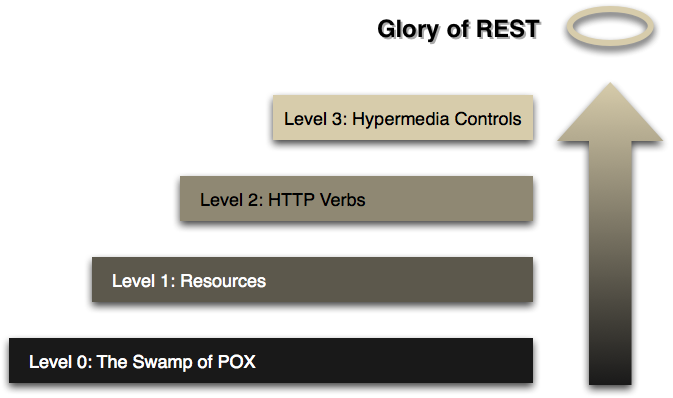
\includegraphics[width=0.6\textwidth]{imagenes/rest-levels}
\caption{Niveles de madurez de una API REST}
\label{fig:niveles-api-rest}
\end{figure}

Nuestra API REST sólo consta de los 3 primeros niveles del modelo de madurez de Richardson. Está implementada en PHP con el framework Slim, que es muy útil cuando se quieren implementar APIs de forma rápida y sencilla. Para el intercambio de datos entre el cliente y el servidor utilizamos el formato JSON (JavaScript Object Notation) que es muy ligero y de gran uso en el intercambio de información vía API REST.\\

Como en el parser, la API REST también hace uso de la base de datos, por lo que también tiene un modelo de datos asociada a ella. Consta de las mismas tablas que en caso del parser, más tres tablas más: User, Competitivity\_graph y Graph\_vertex.

\begin{itemize}
\item \textbf{User}: es la tabla encargada de mantener información de sobre los usuarios que están usando la API REST para subir sus propios rankings y calcular las medidas de competitividad asociadas a esos rankings. Guarda información de el nombre de usuario, la contraseña (cifrada con SHA1), el email, y el apiKey (código alfanumérico que sirve para identificar a un usuario de forma única en la aplicación. Se usa porque REST no tiene estado y es una forma de identificar a los usuarios).

\item \textbf{Competitivity\_graph}: es la tabla que guarda el nombre y las medidas de competitividad asociadas a un grafo de competitividad evolutivo. Las medidas que guarda son el grado medio normalizado (nmd), la fuerza media normalizada (nmd), la eficiencia, la longitud del camino característico (cpl), la tau de Kendall generalizada y el diámetro del grafo.

\item \textbf{Graph\_vertex}: es la tabla que guarda el conjunto de aristas del grafo de competitividad evolutivo. De cada arista se guarda el nodo origen, el destino y el peso de cada arista.
\end{itemize}

El diagrama Entidad-Relación asociado a la API REST se puede ver en la Figura~\ref{fig:er-api}.\\

El diseño completo de la API REST implementada se pueden ver en el Anexo~\ref{app:api-rest}.

\begin{figure}[htb]
\centering
\erapi
\caption{Diagrama E-R asociado a la API REST}
\label{fig:er-api}
\end{figure}


\section{Frontend}

El frontend consiste en una aplicación SPA implementada en AngularJS que se comunica con la API REST comentada anteriormente.\\

La aplicación depende de una serie de módulos Angular que permite una mayor interactividad con el usuario:

\begin{itemize}
\item \textbf{Angular-route}: módulo que permite la definición de nuevas rutas dentro de la aplicación Angular.

\item \textbf{Restangular}: módulo que permite hacer peticiones REST a un servidor.

\item \textbf{Angular-loading-bar}: módulo que permite añadir una barra de carga que indica si una página ha terminado de cargar.

\item \textbf{Angular-chart}: módulo que permite la representación de gráficos. Los tipos de gráficos que soporta son: gráfico de líneas, de radar, de barras y de sectores.

\item \textbf{Cytoscape.js}: módulo que permite representar y analizar grafos.
\end{itemize}

\subsection{Vista de la aplicación}

En esta sección, veremos el aspecto global de la aplicación y las vistas de las que consta ésta.\\

La página de inicio se puede ver en la Figura~\ref{fig:inicio-aplicacion}. En la parte superior, hay una barra de navegación desde la que puede iniciar sesión. En la parte lateral izquierda, se muestran todas las temporadas desde la 1928-1929, hasta la temporada actual y todos los equipos que han jugado en primera división en la Liga. La parte que falta de la pantalla muestra las estadísticas de la temporada actual: clasificación, el histórico de posiciones a lo largo de las jornadas, el grafo de competitividad y distintas medidas de competitividad en forma de gráfico.\\


\begin{figure}[htb]
\centering
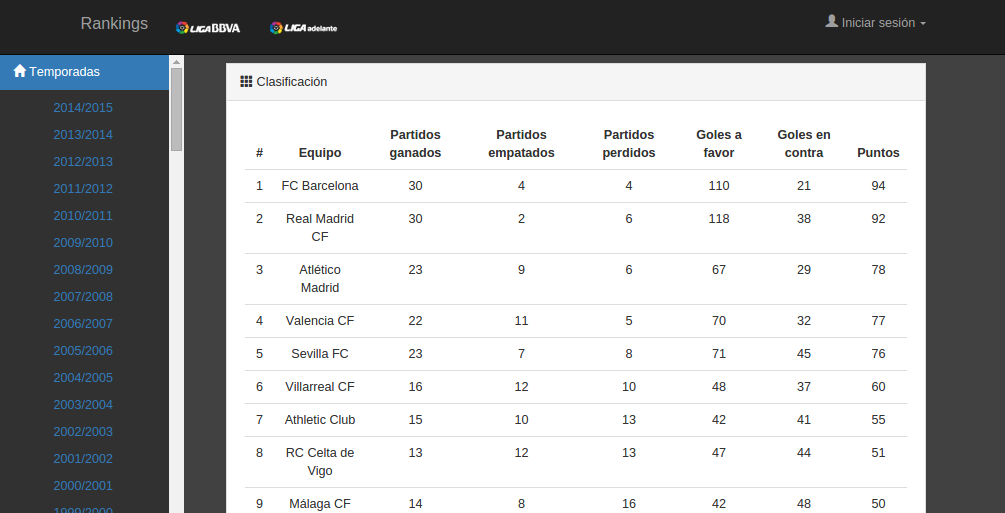
\includegraphics[width=0.9\textwidth]{imagenes/pantallazos-aplicacion/inicio}
\caption{Inicio de la aplicación}
\label{fig:inicio-aplicacion}
\end{figure}

El histórico de posiciones (Figura~\ref{fig:inicio-historico}) muestra, mediante un gráfico de líneas, la posición de cada equipo durante todas las jornadas. Se pueden ver los cambios de posiciones de cada equipo, y las tendencias que siguen a lo largo de la temporada.\\


\begin{figure}[htb]
\centering
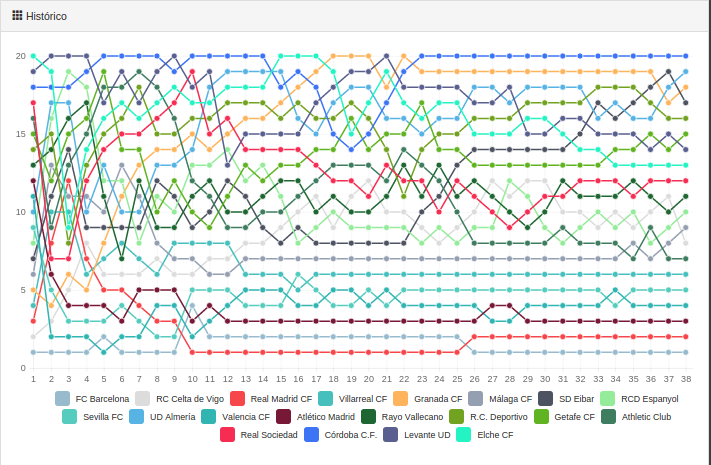
\includegraphics[width=0.9\textwidth]{imagenes/pantallazos-aplicacion/inicio-historico}
\caption{Histórico de posiciones durante la temporada}
\label{fig:inicio-historico}
\end{figure}

Las medidas de competitividad (Figura~\ref{fig:medidas}) se muestran en dos gráficos distintos: el primero de ellos, muestra un gráfico de radar con seis medidas de competitividad (fuerza  y grado medio normalizado, eficiencia, diámetro, longitud del camino característico y tau de Kendall generalizada); en el segundo se muestran las distribuciones acumuladas de la fuerza y del grado normalizado.\\

\begin{figure}[htbp]
\centering
\subfigure[Medidas de competitividad en un gráfico de radar]{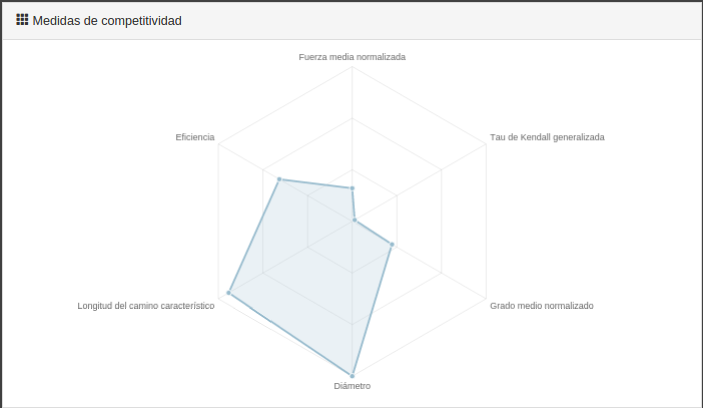
\includegraphics[width=0.45\textwidth]{imagenes/pantallazos-aplicacion/inicio-medidas1}}
\subfigure[Medidas de competitividad en un gráfico de líneas]{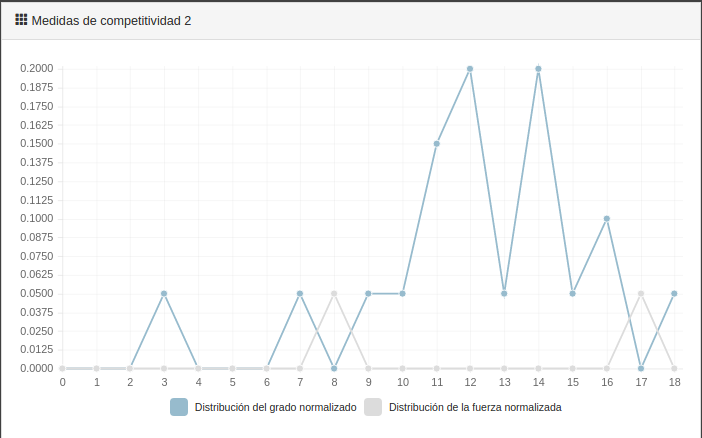
\includegraphics[width=0.45\textwidth]{imagenes/pantallazos-aplicacion/inicio-medidas2}}
\caption{Gráficos con las medidas de competitividad} \label{fig:medidas}
\end{figure}

Por último, en la pantalla de inicio/temporada, se muestra el grafo de competitividad evolutivo (Figura~\ref{fig:inicio-grafo}). Se muestra el grafo junto con los nombres de los equipos, y sus respectivos escudos.\\


\begin{figure}[htb]
\centering
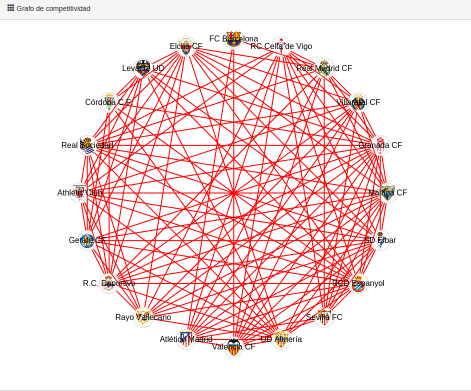
\includegraphics[width=0.9\textwidth]{imagenes/pantallazos-aplicacion/inicio-grafo}
\caption{Grafo de competitividad en la aplicación}
\label{fig:inicio-grafo}
\end{figure}

De la misma forma, si pinchamos sobre un equipo en la pantalla de inicio/temporada nos mostrará información relativa a ese equipo, como escudo y distintas estadísticas. \\

Las primeras estadísticas que se muestran son las relativas al histórico, como goles totales, número de victorias, derrotas y empates, número de temporadas en primera división. Todas estas estadísticas se dan tanto para equipo local como visitante (Figura~\ref{fig:equipo-estadisticas}).\\

\begin{figure}[htb]
\centering
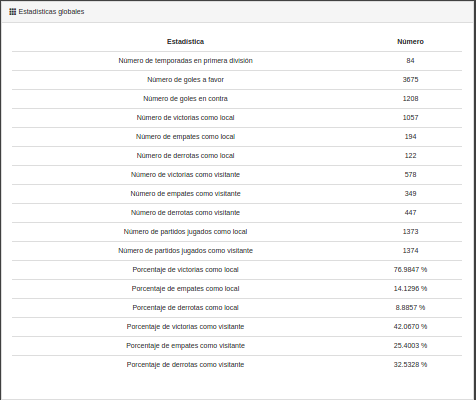
\includegraphics[width=0.9\textwidth]{imagenes/pantallazos-aplicacion/equipo-estadisticas}
\caption{Estadísticas globales de un equipo}
\label{fig:equipo-estadisticas}
\end{figure}

Otras estadísticas que se muestran son los porcentajes de victorias, derrotas y empates tanto como de local como de visitante (Figura~\ref{fig:equipo-local}) en forma de gráfico circular. También se pueden ver los mismos gráficos, pero para goles (a favor y en contra) tanto como local como para visitante.\\

\begin{figure}[htb]
\centering
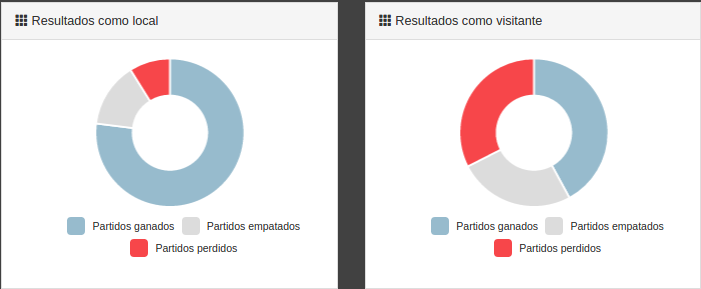
\includegraphics[width=0.9\textwidth]{imagenes/pantallazos-aplicacion/equipo-local}
\caption{Estadísticas de resultados de un equipo}
\label{fig:equipo-local}
\end{figure}

Por último, se muestran las estadísticas por resultados, es decir, se muestran el número de veces que el partido acabó 0-0, 1-0, etc. \\

\begin{figure}[htb]
\centering
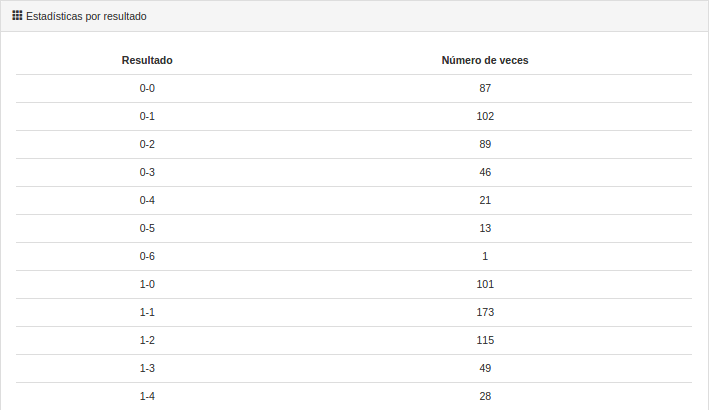
\includegraphics[width=0.9\textwidth]{imagenes/pantallazos-aplicacion/equipo-resultados}
\caption{Estadísticas por resultados de un equipo}
\label{fig:equipo-resultados}
\end{figure}

A parte de ver los resultados de la Liga, también se puede ver el gráfico de competitividad y las medidas para unos rankings de lo que disponga el usuario. Para ello, lo primero que deberá hacer el usuario será registrarse. Para hacerlo, debe ir a \emph{Iniciar Sesión} en la parte superior de la pantalla y pulsar sobre \emph{Registrarse}. Se mostrará un formulario de registro, en el que se deberán rellenar el nombre de usuario, la contraseña y el correo electrónico (Figura~\ref{fig:registro}).\\

\begin{figure}[htb]
\centering
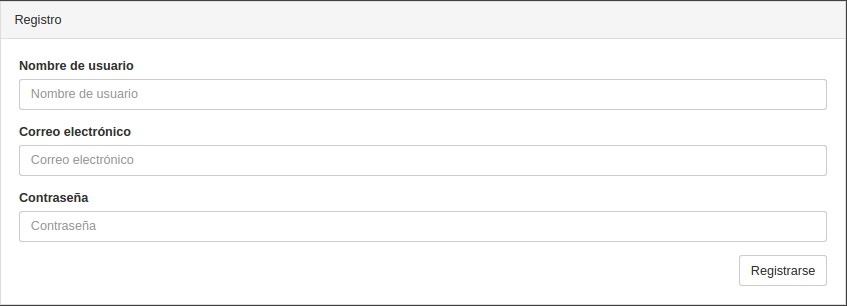
\includegraphics[width=0.9\textwidth]{imagenes/pantallazos-aplicacion/registro}
\caption{Formulario de registro}
\label{fig:registro}
\end{figure}

Una vez rellenos estos datos, nos redirigirá a una nueva página desde la que podremos iniciar sesión. Esta vez sólo nos pedirá el usuario y la contraseña (Figura~\ref{fig:inicio-sesion}). Una vez introducidos los datos de forma correcta, nos llevará a la página de perfil del usuario, en la que se indican todos los rankings que hemos subido.

\begin{figure}[htb]
\centering
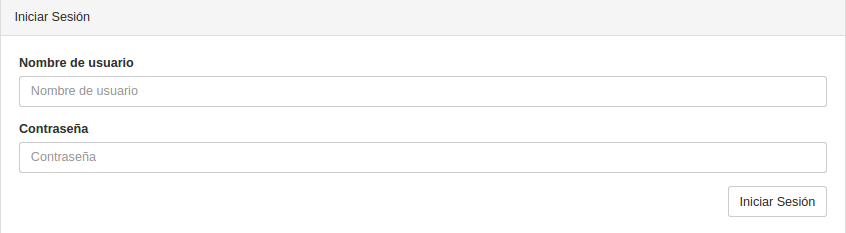
\includegraphics[width=0.9\textwidth]{imagenes/pantallazos-aplicacion/inicio-sesion}
\caption{Formulario para iniciar sesión}
\label{fig:inicio-sesion}
\end{figure}

Para añadir un nuevo ranking, deberemos hacer click sobre el botón \emph{+} que aparece en la parte superior derecha de la página de perfil. Nos mostrará un formulario en el que nos pedirá subir un archivo (Figura~\ref{fig:nuevo-ranking}). \\

\begin{figure}[htb]
\centering
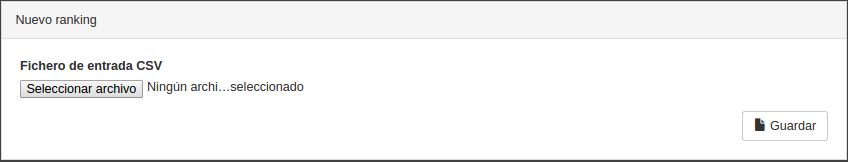
\includegraphics[width=0.9\textwidth]{imagenes/pantallazos-aplicacion/nuevo-ranking}
\caption{Formulario para añadir un nuevo ranking}
\label{fig:nuevo-ranking}
\end{figure}

El fichero que se suba debe tener el siguiente formato:

\begin{minted}{bash}
Nombre del grafo,4,4
RMA,BAR,SEV,VAL
BAR,SEV,VAL,RMA
RMA,BAR,VAL,SEV
RMA,VAL,BAR,SEV
\end{minted}

En la primera línea del archivo, se deben indicar el nombre que llevará ese grafo, el número de equipos y el número de jornadas. Todo ello separado por comas. A partir de la segunda línea hasta el número de jornadas, se deben indicar los nombres de los equipos de izquierda a derecha, donde la izquierda indica mayor posición en el ranking, y la derecha menor posición en el ranking. También deben ir separados por comas.\\

Una vez que se ha cargado el ranking, la aplicación volverá a la página de perfil, donde se mostrará el ranking que se acaba de insertar. Si pinchamos en el nombre de uno de los rankings que acabamos se subir se mostrará el grafo y las medidas de competitividad (Figura~\ref{fig:grafo-medida}). 

\begin{figure}[htbp]
\centering
\subfigure[Grafo de competitividad]{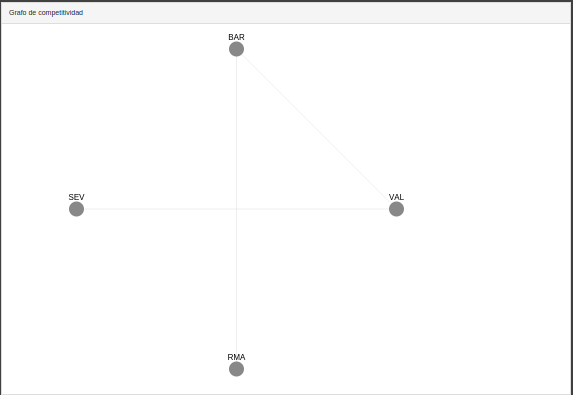
\includegraphics[width=0.9\textwidth]{imagenes/pantallazos-aplicacion/ver-grafo}}
\subfigure[Medidas de competitividad]{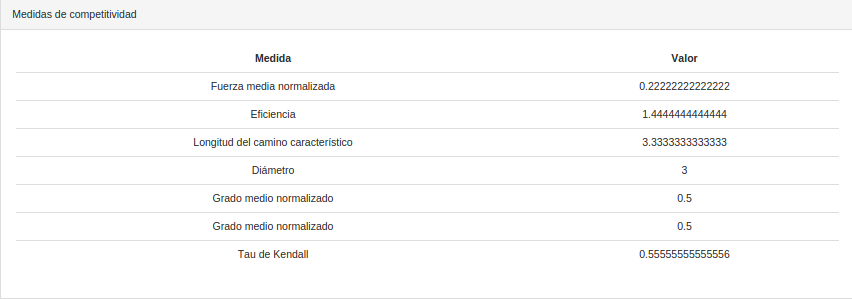
\includegraphics[width=0.9\textwidth]{imagenes/pantallazos-aplicacion/ver-medidas}}
\caption{Grafo y medidas de competitividad}
\label{fig:grafo-medidas}
\end{figure}

\chapter{Aplicación a la temporada 2014-2015 de la liga BBVA}
\chapter{Conclusiones}

Durante esta memoria, hemos visto cómo estudiar la competitividad en una familia de rankings y cómo poder compararlo con otras familias de rankings con la definición de algunas medidas de competitividad como lo son la fuerza y el grado medio normalizado, entre otros.\\

Además, hemos diseñado e implementado una aplicación que extrae datos de la página de la Liga de Fútbol Profesional de todas las temporadas desde 1928 hasta la actualidad y estadísticas de todos los equipos que han jugado en primera división, y calcula el grafo y las medidas de competitividad. Estos datos son intercambiados entre el cliente y el servidor mediante una API REST.\\

Por último, con la ayuda de la aplicación, hemos analizado la competitividad de las últimas cuatro temporadas de la Liga BBVA, quedando como la más competitiva la última disputa, es decir, la temporada 2014-2015.

\section{Mejoras y futuro trabajo}

\begin{itemize}
\item Posibilidad de ver la competitividad a lo largo de las jornadas, es decir, ver las medidas y el grafo de competitividad en una jornada concreta durante la temporada.

\item Añadir un módulo de predicción para ver cómo evolucionará la competitividad a lo largo del tiempo.

\item Posibilidad de implementar una aplicación con Ionic Framework.

\item Añadir un módulo de comparación, que permita comparar dos o más temporadas distintas.

\item Añadir un módulo que permita a los usuarios definir sus propios parsers para añadir nuevas ligas, o incluso, otras temáticas.

\item Mostrar el gráfico histórico de líneas invertido, es decir, que las posiciones más bajas del ranking estén en lo más alto del gráfico.
\end{itemize}


\appendix
\chapter{Diseño de la API REST} \label{app:api-rest}

A continuación se detallan todos los métodos implementados de la API REST: 

\begin{longtable}[c]{@{}ccC{5cm}@{}}
\caption{Métodos de la API REST}\\
\toprule
URL & Método & Descripción\tabularnewline
\midrule
\endfirsthead

\caption{Métodos de la API REST (continuación)}\\
\toprule
URL & Método & Descripción\tabularnewline
\midrule
\endhead

/register & POST & Registra un nuevo usuario\tabularnewline
\hline
/login & POST & Inicio de sesión de un usuario\tabularnewline
\hline
/sport/:sportname/:league/teams & GET & Devuelve los equipos de la liga
:league del deporte :sportname\tabularnewline
\hline
/sport/:sportname/:league/seasons & GET & Devuelve todas las temporadas
de la liga :league del deporte :sportname\tabularnewline
\hline
/sport/:sportname/:league/competitivity & GET & Devuelve las medidas y
el grafo de competitividad de la liga :league del deporte
:sportname\tabularnewline
\hline
/sport/:sportname/:league/measures & GET & Devuelve las medidas de la
liga :league del deporte :sportname\tabularnewline
\hline
/sport/:sportname/:league/clasification & GET & Devuelve la
clasificación de la liga :league del deporte :sportname\tabularnewline
\hline
/sport/:sportname/:league/team/:team & GET & Devuelve información del
equipo :team de la liga :league del deporte :sportname\tabularnewline
\hline
/users/:id/graphs & GET & Devuelve las medidas y el grafo de
competitividad de los rankings subidos por el usuario :id\tabularnewline
\hline
/users/:id/graphs/:graph\_id & GET & Devuelve las medidas y el grafo de
competitividad del ranking :graph\_id subidos por el usuario
:id\tabularnewline
%\hline
/users/:id/graphs/:graph\_id & DELETE & Borra las medidas y el grafo de
competitividad del ranking :graph\_id subidos por el usuario
:id\tabularnewline
\hline
/users/:id/graphs & POST & Añade un nuevo grafo con sus medidas al
usuario :id\tabularnewline

\bottomrule
\end{longtable}
\chapter{Teoría de grafos}

\begin{defi}
Un grafo (o grafo no dirigido) es un par $G = (V,E)$ de conjuntos que satisfacen que $E \subseteq V^2$ y $V \cap E = \emptyset$. Los elementos de $V$ se denominan vértices (o nodos) del grafo $G$ y los elementos de $E$ se denominan arcos (o aristas). Una arista entre los véctices $x, y \in V$ se denota como $xy$ o $yx \in E$.
\end{defi}

La forma usual de representar un grafo es dibujar un punto (o círculo) por cada vértice y unir dos de estos dos puntos (o círculos) con una línea para formar un arco. Cómo estén dibujados los vértices y los arcos es irrelevante. sólo importa qué pares de nodos forman una arista y cuáles no.

\begin{ejemplo}

La Figura \ref{fig:grafo} muestra la representación gráfica de un grafo. Matemáticamente, el grafo es el par $(V, E)$ donde

\[ V = \{A, B, C, D\} \]
\[ E = \{\{A,B\},\{A,C\},\{B,C\},\{C,D\} \} \]

\begin{figure}[htb]
\centering
\ejemplografo
\caption{Ejemplo de grafo}
\label{fig:grafo}
\end{figure}

\end{ejemplo}

\begin{defi}
Se llama orden de un grafo $G$ al número de vértices de dicho grafo. Se denota como $|G|$.\\
Un grafo $G$ se dice que es finito si $|G| < \infty$. Si $|G| = \infty$ se dice que el grafo $G$ es infinito.
\end{defi}

\begin{ejemplo}
El grafo de la Figura \ref{fig:grafo} es un grafo finito, puesto que el número de vértices del grafo es $4$.
\end{ejemplo}

\begin{defi}
Dos vértices $x,y \in V$ del grafo $G = (V,E)$ se dicen adyacentes si existe una arista entre $x$ e $y$ (o $xy \in E$).
\end{defi}

\begin{defi}
Un grafo se dice completo si todos sus vértices son adyacentes.
\end{defi}

\begin{ejemplo}
El grafo de la Figura \ref{fig:grafo_completo} es completo ya que todos sus vértices son adyacentes. En efecto, el vértice $A$ tiene una arista que lo une con los nodos $B$, $C$ y $D$. De la misma forma, se comprueba para los vértices $B$, $C$ y $D$.

\begin{figure}[htb]
\centering
\ejemplografocompleto
\caption{Ejemplo de grafo completo}
\label{fig:grafo_completo}
\end{figure}

\end{ejemplo}

\begin{defi}
Sean $G = (V,E)$ y $G' = (V',E')$ dos grafos. Decimos que $G$ y $G'$ son isomorfos, y escribimos $G \simeq G'$, si existe una biyección $\phi : V \to V'$ tal que $xy \in E \iff \phi(x)\phi(y) \in E' \ \ \forall x,y \in V$. La aplicación $\phi$ recibe el nombre de isomorfismo. Si $G = G'$, $\phi$ se dice que es un automorfismo. 
\end{defi}

Podemos definir operaciones sobre grafos, como la unión o la intersección.

\begin{defi}
Sean $G = (V,E)$ y $G' = (V',E')$ dos grafos, se definen la unión y la intersección de grafos como

\begin{eqnarray*}
G \cup G' := (V \cup V', E \cup E')\\
G \cap G' := (V \cap V', E \cap E')
\end{eqnarray*}

Si $G \cap G' = \emptyset$, entonces $G$ y $G'$ son disjuntos.
\end{defi}

\begin{ejemplo}
La Figura \ref{fig:union_interseccion_grafo} muestra la unión e intersección de grafos. Si $G$ y $G'$ son respectivamente 

\begin{eqnarray*}
G = (\{A, B, C, D, E\}, \{ \{A,B\}, \{B,C\}, \{B,D\}, \{C,E\}, \{D, E\} \})\\
G' = (\{C, D, E, F\}, \{ \{C,D\}, \{C,E\}, \{D,F\}, \{E,F\} \})
\end{eqnarray*}

Por definición,

\begin{multline*}
G \cup G' = (\{A, B, C, D, E, F\}, \{ \{A,B\}, \{B,C\}, \{B,D\}, \{C,E\}, \{D, E\}, \\
\{C,D\}, \{D,F\},\{E,F\} \})
\end{multline*}
\[G \cap G' = (\{C, E\}, \{\{C,E\}\})\]


\begin{figure}[htb]
\centering
\ejemplounionintersecciongrafo
\caption{Ejemplo de unión de unión e intersección de grafos}
\label{fig:union_interseccion_grafo}
\end{figure}

\end{ejemplo}

\begin{defi}

Sean $G = (V,E)$ y $G' = (V',E')$ dos grafos. Si $V' \subseteq V$ y $E' \subseteq E$, se dice que $G'$ es un subgrafo de $G$ (y $G$ es un supergrafo de $G'$).

\end{defi}

\begin{ejemplo}
La figura \ref*{fig:subgrafo} muestra algunos de los subgrafos de $G= (V,E)$ donde

\[ V  = \{A, B, C, D, E\}\]
\[E = \{ \{A,B\}, \{A,C\}, \{A,E\}, \{B,D\}, \{B, E\},\{C,D\}, \{D,E\},\{C,E\} \} \]

Del mismo modo, $G' = (V', E')$ y $G'' = (V'', E'')$ donde

\[ V'  = \{A, B, C, D\}\]
\[E' = \{ \{A,B\}, \{A,C\}, \{B,D\},\{C,D\} \} \]

\[ V''  = \{A, B, C, D, E\}\]
\[E'' = \{ \{A,B\}, \{A,C\}, \{B,D\},\{C,D\},\{B,E\} \} \]

Se ve claramente que $V' \subseteq V$ y $E' \subseteq E$, por lo que $G'$ es un subgrafo de $G$ (o $G$ es un supergrafo de $G'$). Análogo para $G''$.


\begin{figure}[htb]
\centering
\ejemplosubgrafo
\caption[Ejemplo de subgrafos de un grafo]{Ejemplo de subgrafos de un grafo $G$}
\label{fig:subgrafo}
\end{figure}

\end{ejemplo}

\begin{defi}
Sea $G = (V,E)$ un grafo (no vacío). El grado de un vértice $v \in V$, denotado por $d_G(v) = d(v)$, se define como el número de vértices adyacentes a $v$.\\

Si todos los vértices de $G$ tienen el mismo grado $k$, el grafo $G$ es regular.
\end{defi}

\begin{defi}
Se define el grado medio de un grafo $G = (V,E)$ como el número

\begin{equation}
d(G) = \dfrac{1}{|V|} \sum_{v \in V} d(v)
\end{equation}
\end{defi}

\begin{defi}
Un camino es un grafo no vacío $P = (V, E)$ de la forma

\begin{equation*}
V = \{ x_0,x_1,\dots,x_k\} \quad \quad E = \{ x_0 x_1, x_1 x_2, \dots, x_{k-1}x_k \}
\end{equation*}

donde $x_i \neq x_j \ \forall i \neq j$.\\

Los vértices $x_0$ y $x_k$ se denominan final del camino $P$. Los vértices $x_1, \dots, x_k$ se denominan vértices interiores del camino $P$.\\

El número de aristas del camino se denomina longitud del camino.
\end{defi}

\begin{defi}
Un grafo no vacío $G$ se dice conexo si cualquier par de vértices están unidos por un camino de $G$.
\end{defi}

\begin{defi}
Sea $G = (V,E)$ un grafo. Un subgrafo conexo maximal de $G$ se llama componente conexa de $G$.
\end{defi}

\begin{defi}
Un clique es un conjunto de nodos mutuamente conectados entre sí.
\end{defi}

\begin{ejemplo}
Un triángulo es un clique formado por tres nodos.
\end{ejemplo}

\begin{defi}
Un grafo dirigido (o digrafo) es un par $(V,E)$ de conjuntos disjuntos (de vértices y de aristas) junto con dos funciones $\mathrm{init} : E \to V$ y $\mathrm{ter} : E \to V$ que asigna a cada arista $e$ un vértice inicial $\mathrm{init}(e)$ y un vértice terminal $\mathrm{ter}(e)$.\\

La arista $e$ se dice dirigida desde $\mathrm{init}(e)$ hasta $\mathrm{ter}(e)$.\\

Si $\mathrm{init}(e) = \mathrm{ter}(e)$, la arista $e$ se dice que es un bucle.
\end{defi}

\begin{ejemplo}
La Figura \ref*{fig:grafo_dirigido} muestra la representación gráfica un grafo dirigido. Matemáticamente, es el par $(V,E)$ donde

\[V  = \{A, B, C, D\}\]
\[E = \{ \{A,B\}, \{A,C\}, \{C,C\},\{B,C\}, \{C,D\} \} \]

junto con las funciones $\mathrm{init} : E \to V $ y $\mathrm{ter} : E \to V$ definidas de la siguiente manera:

\begin{center}
\begin{tabular}{l|r}
\begin{tabular}{r c c c}
$\mathrm{init}:$ & $E$ & $\to$ & $V$\\
			     & $\{A,B\}$ & $\mapsto$ & $A$\\
			     & $\{A,C\}$ & $\mapsto$ & $A$\\
			     & $\{C,C\}$ & $\mapsto$ & $C$\\
			     & $\{B,C\}$ & $\mapsto$ & $B$\\
			     & $\{C,D\}$ & $\mapsto$ & $C$\\
			      
\end{tabular} &
\begin{tabular}{r c c c}
$\mathrm{ter}:$ & $E$ & $\to$ & $V$\\
			     & $\{A,B\}$ & $\mapsto$ & $B$\\
			     & $\{A,C\}$ & $\mapsto$ & $C$\\
			     & $\{C,C\}$ & $\mapsto$ & $C$\\
			     & $\{B,C\}$ & $\mapsto$ & $C$\\
			     & $\{C,D\}$ & $\mapsto$ & $D$\\
			      
\end{tabular} 
\end{tabular}
\end{center}

Además la arista $\{C,C\}$ es un bucle porque $\mathrm{init}(\{C,C\}) = \mathrm{ter}(\{C,C\}) = C$.

\begin{figure}[h]
\centering
\ejemplografodirigido
\caption{Ejemplo de grafo dirigido con bucle}
\label{fig:grafo_dirigido}
\end{figure}

\end{ejemplo}

\begin{defi}\label{def:orientacion}
Un grafo dirigido $D = (V', E')$ es una orientación de un grafo (no dirgido) $G = (V,E)$ si $V = V'$ y $E = E'$ y $\{\mathrm{init}(e), \mathrm{ter}(e) \} = \{x,y\} \ \forall e = xy \in E$.
\end{defi}

\section{Algunos tipos de grafos}

\begin{defi}
Un grafo ponderado es un grafo con una función $\mathrm{w} : E \to \R$, es decir, que $\mathrm{w}$ asocia un número real a cada arista. Esta función recibe el nombre de función peso.
\end{defi}

\begin{ejemplo}
El grafo $G = (V,E)$ con 

\begin{eqnarray}
V = \{A, B, C\}\\
E = \{ \{A,B\}, \{A,C\}, \{B,C\} \}
\end{eqnarray} 

es un grafo. Si le añadimos la función $\mathrm{w} : E \to \R$ definida de la siguiente forma, $G$ es un grafo ponderado (ver Figura \ref{fig:grafo_ponderado}).

\begin{equation*}
\begin{tabular}{r c c c}
$\mathrm{w}:$ & $E$ & $\to$ & $\R$\\
			     & $\{A,B\}$ & $\mapsto$ & $e$\\
			     & $\{A,C\}$ & $\mapsto$ & $5$\\
			     & $\{B,C\}$ & $\mapsto$ & $\pi$
			      
\end{tabular}
\end{equation*}
\begin{figure}[htb]
\centering
\ejemplografoponderado
\caption{Ejemplo de grafo ponderado}
\label{fig:grafo_ponderado}
\end{figure} 
\end{ejemplo}

\begin{defi}
Dado un grafo ponderado $G = (V,E)$ y $\mathrm{w} : E \to \R$, decimos que una arista $e \in E$ incide en el vértice $v \in V$, si $\mathrm{ter}(e) = v$. 
\end{defi}

\begin{defi}
La fuerza de un vértice en un grafo ponderado se define como la suma de todos los pesos de sus aristas incidentes.
\end{defi}

\begin{defi} \label{def:dominancia}
Un grafo de dominancia $G=(V,E)$ es un grafo dirigido tal que para todo $x,y \in V$ se cumple una de las dos condiciones siguientes, pero no ambas simultáneamente:

\begin{itemize}
\item $\mathrm{init}(xy) = x$ \quad y \quad $\mathrm{ter}(xy) = y$
\item $\mathrm{init}(xy) = y$ \quad y \quad $\mathrm{ter}(xy) = x$ 
\end{itemize}
\end{defi}

\begin{ejemplo}
Si consideramos el grafo de la Figura \ref{fig:grafo_dominancia}, vemos que para todo vértice $x,y \in \{A, B, C, D\}$ se cumple alguna de las dos condiciones anteriores, pero no ambas simultáneamente. Por ejemplo, para los vértices $A, D$ se cumple que $\mathrm{init}(\{A,D\}) = A$ y $\mathrm{ter}(\{A,D\}) = D$, pero no se cumple la otra condición. De la misma se comprueban los vértices restantes.   

\begin{figure}[h]
\centering
\ejemplografodominancia
\caption{Ejemplo de grafo de dominancia}
\label{fig:grafo_dominancia}
\end{figure}
\end{ejemplo}

\begin{defi}
Llamamos grafo complementario de $G = (V,E)$, y lo denotamos como $\overline{G}$ al grafo que tiene como conjunto de vértices $V$ y como conjunto de aristas, las aristas que no están unidas de $G$.
\end{defi}

\begin{ejemplo}

La Figura~\ref{fig:grafo_complementario} muestra un grafo $G$ y su correspondiente grafo complementario $\overline{G}$. Las aristas que no están unidas en $G$, sí lo están en $\overline{G}$.

\begin{figure}[h]
\centering
\ejemplografocomplementario
\caption{Ejemplo de grafo complementario}
\label{fig:grafo_complementario}
\end{figure}
\end{ejemplo}
\end{ejemplo}
\chapter{Manual de instalación}

Para instalar la aplicación necesitaremos seguir los siguientes pasos\footnote{De ahora en adelante, supondremos que estamos en un entorno Linux (en particular, un entorno Ubuntu o derivados)}:

\begin{enumerate}
\item Instalar las dependencias con los siguientes comandos:

\begin{minted}{bash}
sudo apt-get install apache2
sudo apt-get install php5 php5-cli php5-mysql
sudo apt-get install php5-curl
sudo apt-get install mysql-client mysql-server
\end{minted}

Durante la instalación de la última dependencia se nos pedirá la contraseña del usuario \emph{root} de la base de datos MySQL.

\item Creación de un nuevo usuario para la base de datos. 

Entramos en MySQL con como root con el comando

\begin{minted}{bash}
mysql -u root -p
\end{minted}

Nos pedirá la contraseña del usuario \emph{root} que hemos configurado durante el paso anterior.

\begin{enumerate}
\item Escribimos el siguiente comando para crear un nuevo usuario:

\begin{minted}{sql}
CREATE USER 'rankings'@'localhost' IDENTIFIED by '1234';
\end{minted}

donde \emph{1234} es la contraseña del usuario \emph{rankings}.
\end{enumerate}

\item Habilitar el módulo \emph{mod\_rewrite} de Apache.

\begin{enumerate}
\item Escribimos los siguientes comandos en la Terminal

\begin{minted}{bash}
sudo a2enmod rewrite
sudo service apache2 restart
\end{minted}


\item Ejecutamos los comandos

\begin{minted}{bash}
sudo nano /etc/apache2/sites-available/default
\end{minted}

y buscamos en el archivo \emph{<Directory /var/www/>}.

\item Sustituimos el contenido de \emph{<Directory /var/www/>} por lo siguiente

\begin{minted}{bash}
<Directory /var/www/>
      Options Indexes FollowSymLinks MultiViews
      # changed from None to FileInfo
      AllowOverride FileInfo
      Order allow,deny
      allow from all
</Directory>
\end{minted}

\item Reiniciamos Apache con

\begin{minted}{bash}
sudo service apache2 restart
\end{minted}

\end{enumerate}

\item Instalación de Bower

\begin{enumerate}
\item Descargar node desde su página oficial \url{https://nodejs.org}
\item Instalar npm (si no viene instalado junto a node)
\item Ejecutar el comando 

\begin{minted}{bash}
npm install -g bower
\end{minted}

\item Para comprobar que tenemos instalado Bower ejecutar 

\begin{minted}{bash}
bower -v
\end{minted} 

Si nos aparece el número de versión, está instalado.

\item Ir a la carpeta web y ejecutar el comando 

\begin{minted}{bash}
bower install
\end{minted} 

Nos instalará todas las dependencias necesarias.
\end{enumerate}

\item Instalación de Composer

\begin{enumerate}
\item Ejecutar los siguientes comandos

\begin{minted}{bash}
curl -sS https://getcomposer.org/installer | php
mv composer.phar /usr/local/bin/composer
\end{minted} 

\item Ir a la carpeta \emph{web} y ejecutar el comando 

\begin{minted}{bash}
composer install
\end{minted}

Nos instalará todas las dependencias necesarias.

\end{enumerate}

\item Creación de las tablas de la base de datos y carga de los datos

\begin{enumerate}
\item Vamos a la carpeta \emph{parser} y escribimos

\begin{minted}{bash}
mysql -u rankings -p
source rankings.sql
source datos.sql
\end{minted}

\end{enumerate}

\item Movemos la carpeta de la aplicación hacia la carpeta \emph{var/www/html} del servidor Apache.

\item Abrimos un navegador y escribimos \emph{localhost}. Si todo ha ido bien, tendremos la aplicación funcionando.

\end{enumerate}


\backmatter
\nocite{*}
\bibliographystyle{bibliografia/apalike-es}
\bibliography{bibliografia/bibliografia}

\end{document}